\begin{solution} Ý tưởng chính là viết ánh sáng phân cực phẳng như sự chồng chất của hai sóng ánh sáng phân cực tròn có cùng tần số. Ý tưởng chính là viết ánh sáng phân cực phẳng như sự chồng chất của hai sóng ánh sáng phân cực tròn có cùng tần số.
\begin{center}
    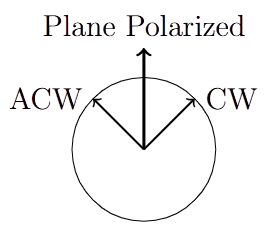
\includegraphics[width=0.25\textwidth]{solutions/figures/polarization-decomposition.png}
\end{center}
    
Sau khi đi qua dung dịch, do chúng có chỉ số khúc xạ khác nhau là $n_L$ và $n_R$, độ chênh lệch pha giữa chúng được cho bởi
$$\frac{\phi}{2\pi} = \frac{L}{\lambda_{\text{medium}}} = \frac{L}{\frac{\lambda}{n}} \implies \Delta \phi = \frac{2\pi}{\lambda}L\Delta n.$$
    
Tuy nhiên, cần lưu ý rằng đây là độ dịch pha chứ không phải góc quay.

\begin{center}
    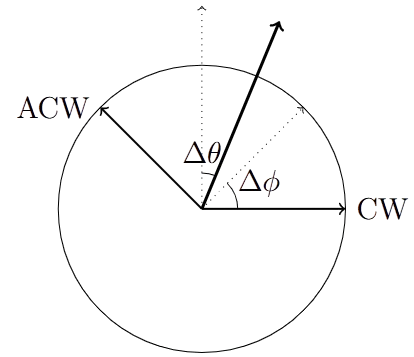
\includegraphics[width=0.3\textwidth]{solutions/figures/rotation-shift.png}
\end{center}
    
Do đó $\Delta \theta = \frac{1}{2}\Delta \phi = \frac{\pi}{\lambda} L \Delta n$. Thay các giá trị vào ta được $\boxed{\Delta \theta = \frac{3\pi}{2} \approx 4.71\;\mathrm{rad}}$.

\end{solution}
